\chapitre{Du manger mou aux nouvelles, le mardi 19 juillet 2033}{Trop «timoroso»,}{ avait dit l’inimitable Alessandro Costi. Trop poltron, trop pissou, trop chie-en-culotte ! Il est vrai que Timothée ne s’accordait pas grand mérite du côté bravoure. Quand on passe une partie de sa vie à longer les murs ou à marcher en fixant le trottoir, on n’apprend pas à braver les affreux, à défendre ses pieds carrés, à faire sa place sous le soleil du petit Bon Dieu. On ne devient jamais audacieux au point d’ajouter quatre cordes supplémentaires à sa lyre pour l’imposer aux quatre coins cardinaux. }

On se contente de faire le moins de couacs possible avec un trombone qu’on déteste, qu’on nous a forcé dans la gorge à grands coups de masse. On suit sa partition sans maugréer, après, on essaie de filer sans se faire voir. On refoule quotidiennement l’envie d’envoyer paître l’affreuse mégère qui bat la mesure entre deux cuissons de confiture aux cerises. Timothée de Milet n’a sûrement pas eu de mère. Ou s’il en a eu une, elle est disparue alors qu’il était nourrisson. Assis dans son officine le moral en compote pour cause de souvenirs recensés, le fils de la Maririou ne remarque pas tout de suite la stature massive de Robespierre Alcide qui occupe son cadre de porte.

- À ta question d’hier, j’ai une question.

Timothée lève la tête.

- T’en veux combien ?

Il est direct ce matin, le collègue !

- Euh… deux ? C’est-y compliqué ?

Robespierre lui lance une petite bouteille de Tylenol en le gratifiant d’un clin d’œil.

- Attrape, y en a justement deux là-dedans.

Et il disparaît avant que le CS-1 puisse dire quoi que ce soit, dire quelque chose comme “merci infiniment !”, ou comme “bonne idée d’avoir mis ça dans une bouteille vide de pilules; ça va mieux passer devant les détecteurs d’objets”, ou comme “laisse faire, l’idée me rend insomniaque”, ou comme “en aurais-tu une troisième ?”.

Mais, à bien y penser, comment le gaillard a-t-il su qu’il en fallait deux ? Se douterait-il de quelque chose ? Personne n’est au courant ! Personne ne doit l’être ! Reste que la question est maintenant de savoir comment refiler cette «solution» à ses parents. Comment avoir le courage de le faire. Comment ne pas être «timoroso» ! Y en a-t-il seulement d’autres, de solutions ? Les génératrices à espoir, les matrices à espérance, les dynamos à lumière-au-bout-du-tunnel, étaient toutes tombées en panne depuis belle lurette et Timothée avait été recalé au certificat en technique jovialiste. Depuis que la société, essentiellement faite de brutes grégaires, était devenue folle, folle et impitoyable, plus que jamais, la pilule du bonheur représentait une avenue moralement défendable. Encore fallait-il pouvoir la présenter, la soutenir, l’administrer. Assistance à deux suicides ? Meurtres par compassion avec circonstances atténuantes ? Euthanasie avant l’état grabataire ? L’être humain n’a-t-il pas le droit de décider d’aller voir ailleurs quand il s’emmerde dans une grisaille sans pitié, sans gratifications, sans améliorations possibles ?

- Chiennerie !

Mais pour l’instant, il doit descendre à la cafétéria son tube de Tylenol en poche. Une note de service de Carl Michaud, l’inquiétant directeur général du Centre, lui en a intimé l’obligation. C’est en fait une journée dont le grand patron pourrait se passer. Il lui faut en effet accueillir Ti-Dédé, c’est-à-dire T.I.D.D. ou Thierry-Ian Dennis-Dubeau, le chef des Verts et chef de l’opposition à Québec. Flairant des élections à l’automne, l’homme politique parcourt le Québec en quête de munitions et de plates-formes pour tester quelques ballons d’essai. Son ambition ? Devenir le premier Vert de l’histoire à diriger le Québec. Rien de moins ! 

\begin{floatingfigure}[l]{40mm}
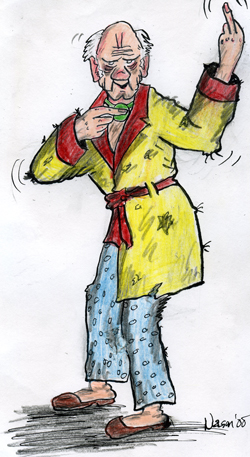
\includegraphics[height=60mm]{corps/chapitre6/img/personnage-vader.jpg}
\end{floatingfigure}

Au moment où Ti-Dédé fait son entrée dans l’établissement, Philippe «Flipper» Dauphin jette un dernier coup d’œil à la cafétéria. Directeur des communications et âme damnée de Carl Michaud, sa mission est de réduire tant qu’il le peut tout potentiel de retombées négatives. Apercevant Dart Vader assis avec les quatre pensionnaires en 2P (salles communautaires pour personnes autonomes) choisis minutieusement par lui-même, Flipper le fait chasser in extremis par ses deux adjoints en uniforme de la Sécu, deux gorilles épouvantables.

- J’ai autant le droit qu’eux autres à être ici, moi, métallise-t-il de sa canule.

Mais rien n’y fait. Les sbires du Flipper l’entraînent vers la sortie. Il faut dire que le sieur Dauphin sait s’entourer. Les horribles frères «Papynut» et «Bluesly» Côté sont habituellement gardés au sous-sol en tant que geôliers. Comme les employés du Centre n’arrivaient pas à les départager, on en était venu à les appeler «PapyBlues». On disait, par exemple, «Je descends chez les PapyBlue !» ou «Penses-tu sérieusement que les PapyBlues s’adonnent à la torture ?» ou «Madame Thériault, si vous n’arrêtez pas de tanner madame Labbée, je vais vous amener chez les PapyBlues !». Avec le temps, les abominables frangins dont les sobriquets remontaient à leur jeunesse de hockeyeurs semi-professionnels avaient appris à ne pas poser de questions, ce qu’ils faisaient très bien.

Grand, distingué, affable, habillé en carte de mode, Ti-Dédé, suivi de son escorte, des patrons du Centre et d’une petite horde de journalistes, serre des mains ici et là au hasard de sa promenade dans les zones autorisées du rez-de-chaussée dont fait partie la cafétéria. Sans surprendre personne, il y entre et s’approche d’une table où quatre bons vieux qu’on a astiqués et mis en scène viennent soi-disant de finir leur ration de Nutrisuz, sourire aux lèvres. Adoptant cet air sérieux que les politiciens doivent afficher quand il faut dénoncer une iniquité, le chef politique fait face aux représentants des médias.

- Mesdames et messieurs les journalistes, je me demandais, en entrant ici, si mon bon ami monsieur Michaud, le souriant directeur général de cet établissement ultra moderne, ne pourrait pas nous faire servir, à chacun d’entre nous, personnel politique, fonctionnaires du MAG ou journalistes, une portion de Nutrisuz, ce brouet que tout le monde, ici, appelle «manger mou». Ainsi, à l’heure où des débats ont cours sur la nature de ce produit et sur ses conséquences sur la santé publique, nous serions plus en mesure de pouvoir nous en faire une opinion. Qu’en pensez-vous, cher ami ?

Carl Michaud avait prévu le coup et fait un signe de tête à Amédée Chicot qui, aidé de Simon Saint-Pierre, passe à l’action. En moins de deux minutes, tous les visiteurs se sont fait remettre par un «bénévole» empathique, un contenant d’ABS chaud empli de Nutrisuz à saveur de fruits de mer à l’ail. Pas si mal pour un petit mardi de semaine au tout début de l’avant-midi !

- Il y a des breuvages disponibles à la fontaine, eau, limonade ou thé, fait remarquer Michaud à voix haute. Demandez à nos sympathiques bénévoles, ils vous fourniront le contenant nécessaire.

Ostensiblement, Dennis-Dubeau n’apprécie pas son plat et, mimiques à l’appui, il semble questionner son entourage où, selon toute vraisemblance, un consensus est en train de s’établir à l’effet que cette nourriture est une honte. Ici et là, des journalistes y trempent le bout des lèvres et se regardent les uns en riant, d’autres en grimaçant. Voilà plus qu’il n’en faut pour que le politicien reprenne la parole.

- Mesdames et messieurs les journalistes, si vous voulez bien me permettre d’interrompre votre succulent repas, je ne serai pas long.

Même si les rires escomptés font défaut, le tribun lève les deux bras.

- Mesdames et messieurs, vous goûtez présentement à cette bouette infâme que nous, la société québécoise porteur de ce flambeau allumé il y a 500 ans par un navigateur breton appelé Jacques Cartier, que nous, dis-je, servons à nos aînés, à ceux-là même, à celles-là mêmes, qui ont façonné le Québec moderne dans lequel nous évoluons tous et toutes. Ce concentré de produits chimiques importés des États-Unis au mépris des quotas de gaz à effet de serre, est une aberration à laquelle nous les Verts, allons nous attaquer dès le lendemain de notre prise du pouvoir, si jamais le premier ministre a le courage, je dis bien le courage, de déclencher des élections ! Nos aînés méritent de manger de la vraie nourriture, pas un résidu de compote électrochimique. Vous croyez que j’exagère ? Que je parle en politicien ? Portez plutôt attention à la liste des éléments de base du cocktail que l’on fait ingurgiter à nos pères et à nos mères.

Il a mis ses lunettes et a ouvert un calepin.

- Je vous traduis ce qu’on peut lire en anglais, et uniquement en anglais, ce qui, soit dit en passant, est un accroc à nos lois, sur la boîte d’emballage:

    Protéines 15% à 30% : poudre de petit lait et/ou albumine et/ou isoflavones du soya, acides aminés essentiels (tryptophane, lysine, méthionine, phénylalanine, thréonine, valine, leucine et l’isoleucine)

    Lipides 28% à 38% : huile végétale (huile de soya et/ou de carthame et/ou de canola), acides gras mono et polyinsaturés, acides gras essentiels (acide linoléique, acide linolénique)

    Glucides 40% à 55% : glucose, fructose, maltodextrines, amidon de maïs, pectines

    Fibres de fruits et légumes, multivitamines et minéraux

    Additifs pour la conservation : acide sorbique, acide benzoïque, sulfites, acide malique, ascorbates, gallates, acide nicotinique, agar-agar, gomme de guar, sorbitol, mannitol, monodiglycérides, cellulose, acide stéarique, acide glutamique, glutamates, acide inosinique, azoformamide…

    Arômes et colorants artificiels.

- Et j’en passe des plus difficiles à prononcer.

La salle sourit.

- Et, en petits caractères, un peu plus bas, on retrouve cette inquiétante mention:

    Peut contenir des produits génétiquement modifiés.

Un grand silence s’est établi.

- Y a quand même une bonne nouvelle, le Nutrisuz ne contient ni lactose, ni gluten et il est faible en gras saturés.

Quelques rires fusent. Ti-Dédé semble s’être rallié les scribes.

- Mesdames et messieurs, on est en train de transformer nos aînées en machines de laboratoires. On est en train de les empoisonner à petit feu sous prétexte d’économies. Il existe pourtant des rapports produits aux Nations Unies et à l’Organisation mondiale de la santé, depuis une vingtaine d’années sur les impacts sociosanitaires des substances génétiquement modifiées. Et je ne vous parle pas de ces études plus récentes, plus inquiétantes encore, comme celles qui ont cours présentement en Californie où on est en train d’établir des rapprochements significatifs entre la diminution alarmante de l’espérance de vie chez nos aînés et l’absorption de Nutrisuz avec son cocktail d’OGM.

Les journalistes grafignent leurs notes comme s’ils ne craignaient pas la tendinite.

- Nous du Parti Vert, nous disons «Assez !». Ce n’est pas une façon de traiter les gens, à plus forte raison ceux à qui nous devons tout ! Je m’engage devant vous à ce que le jour même où nous prendrons le pouvoir, nos vieux puissent recommencer à manger sans s’empoisonner, à manger dans la dignité. Comme ces hommes et ces femmes le dirent si bien à l’époque où ils étaient de jeunes adultes fonçant pour faire du Québec un état moderne n’ayant rien à envier aux autres, «le mépris n’aura qu’un temps !» Merci mesdames et messieurs.

Jugeant qu’il en avait dit assez pour satisfaire à toutes les exigences des différents bulletins de nouvelles, le chef de l’opposition s’assoit sur le coin d’une table et liquide une communication acheminée à sa boucle d’oreille. En même temps, des journalistes l’approchent pour les entrevues, raisons d’être de son déplacement. Parmi eux, subreptice, Dart Vader s’avance par reptation calculée. Ce que voyant, Timothée qui n’avait osé pénétrer dans la salle, sourit et fait volte-face. Heureusement pour Dennis-Dubeau !

Car dans le grand couloir, la porte de l’ascenseur s’ouvre et Luce Morency aussi nue et confuse que d’habitude, en sort comme s’il était normal qu’il en soit ainsi. Pire, elle n’est qu’à cinq pas de l’entrée de la cafeteria. Sans perdre un instant, le CS-1 démarre son bruyant Saguewanish et fonce vers elle.

- Oups oups oups ! Attendez un p’tit peu, madame Morency, vous pouvez pas vous rendre b’en loin comme ça, vous allez attraper le rhume.

- Le rhume ?

- Allô ! 6 Nord ! Code magenta ! 6 Nord ? Allô ? Code Magenta.

Quelqu’un finit par répondre.

- Je vous remonte, madame Morency. Elle a failli débarquer dans la conférence de presse de Dennis-Dubeau. Non. Elle a pas de vêtements. Ne-non, je ne blague pas !

- On arrive.

- Non, y a trop de monde dans le coin. Je vous la monte.

- OK !

Un grand six pieds à la barbe poivre et sel, les mains appuyées au fond des poches de son sarrau blanc, a remarqué la commisération de Timothée.

- Qui c’est ?

- C’est rien de bien grave, docteur Bellavance, répond-il en pitonnant l’ascenseur. C’est une 3P-M en assez bonne santé et pas méchante du tout.

- N’ayez crainte, je ne fais pas de recrutement pour ma ferme hormonale, ironise le chercheur. Mais faudrait peut-être la couvrir.

Sans hésitation, il retire son sarrau et le tend à Timothée qui en revêt Luce Morency.

- Merci docteur, c’est gentil.

- C’est une de vos administrées ?

- Non, mais je vais la reconduire. On peut pas la laisser de même. Venez Mme Morency, l’ascenseur est arrivé.

- Et mon survêtement, il s’en va où ?

- Au 6e Nord. Mais je vais leur dire de vous le ramener.

Le regard que le sinistre homme de science avait posé sur la démente n’était pas sans rappeler celui d’un boa constrictor en train de lorgner une innocente chevrette, une pensée que Timothée, de retour à son étage, se dépêche de chasser.

Comme il arrive au poste de garde, il remarque que Laurent Bérubé y est assis, des écouteurs sans fil aux oreilles. En voyant son supérieur, il se lève et file sur sa trottinette, le gratifiant d’un sourire méchant. Le CS-1 pourrait lui ordonner de revenir, l’obliger à retirer son casque d’écoute, lui réexpliquer le règlement. Mais il laisse tomber et continue jusqu’à son bureau, méditant sur la sournoiserie du gaillard qui pourrait très bien être un de ceux qui auraient pu saboter sa Saguewanish. Timothée double tape son dispositif personnel polyvalent.

- Atelier mécanique !

La sonnerie se fait entendre une dizaine de coups avant qu’on ne réponde.

- Atelier mécanique, bonjour.

- Ma Saguewanish va mal, je voudrais la faire vérifier.

- A va mal comment ?

- Il y a comme un bruit…

- Quelle sorte de bruit ?

- Quand je roule, tout le monde arrête de parler pour me regarder passer …

- A sent-y le diable ?

- Aucune senteur, juste un gros bruit de plus en plus agressant.

- Va falloir l’inspecter. C’est à quel nom ?

- Timothée Tardif.

- Ah ! Le Motté ! C’est beau ! Amène-la !

Une voix monocorde de fond-de-cacane lui fait momentanément oublier ses ennuis mécaniques. Dart Vader vient d’appuyer sur la valve de phonation fixée à sa canule.

- J’ai réussi à parler à Ti-Dédé, chef. Je lui ai dit que j’avais tout le temps faim et que j’haïssais le manger mou.

Timothée ne bronche pas.

- J’ai dit aussi que ça me donnait des coliques. Normalement, je vas passer aux nouvelles.

- J’ai rien entendu, Monsieur Gagnon, et je veux rien entendre.

- C’est juste que tes boss, i’ vont me haïr, chef !

Et le bonhomme de s’esclaffer en émettant d’horribles sons, ce qui amuse Jean Saint-Gelais, un pensionnaire ridé comme peau de chagrin, qui s’adonne à rôder aux alentours sans faire de bruit, tel le vrai malfaiteur qu’il est.

- Dart Vader, t’es mon héros, clame-t-il. Une chance que t’es là, man ! Lâche pas !

Encore une fois, remarque Timothée, le tout nouveau progiciel de gestion est hors service, comme c’est le cas de plus en plus souvent depuis le début. Depuis que l’Association des centres régionaux de gériatrie du Québec (ACRGQ), en partenariat avec un gros fournisseur de solutions établi à Montréal, ont opté pour une plate-forme Linux, l’impressionnante SUSE 256 bits de Novell, et l’ont implanté partout au Québec.

- C’est un bogue intermittent qu’ils n’arrivent pas à découvrir, avait-il expliqué, la semaine dernière, à Pierre Asselin, un vieil ingénieur logiciel quasi aveugle placé dans une salle pour personnes en perte d’autonomie, une 3P-M.

Contrairement au règlement, Le CS-1 l’avait fait entrer dans son coqueron de bureau et l’avait aidé à s’asseoir devant son terminal.

- Les bogues intermittents sont les pires à régler, avait soutenu l’informaticien ses pauvres yeux rivés sur l’écran. Ou le problème est matériel, une composante, un circuit, une rainure, une faiblesse, ou il est logiciel, une incompatibilité, une erreur d’écriture, une bêtise de programmation.

- Tout a beau être Open Source, ça plante, plante et replante. Carl Michaud est à la veille de faire assassiner Vlado Marcovsky.

- Qui est-ce ?

- Son directeur de l’informatique.

Et cette semaine, on dirait que c’est pire encore. Incompatibilité avec certaines puces ? Mauvaises intégrations de fonctions complémentaires ? Routines non prévues dans le système d’exploitation ? Personne ne le sait. Pourtant, chez lui, Timothée n’a pas de problème. Évidemment, les équipements ont de l’âge. Il en est encore à un vieux système Microsoft 3D à 128 bits où, à défaut de vitesse, la stabilité est remarquable.

Le CS-1 en profiter pour y regarder ce que les médias ont fait des propos du chef des Verts, un politicien qui ne saura jamais quelle veine il a eu tout à l’heure et quelle chandelle il doit à un «obscur binoclard bedonnant sans blonde cassé comme un clou en train de devenir chauve». Partout, à ce qu’il semble, en furetant d’une chaîne à l’autre, le manger mou fait la UNE. On voit l’homme politique le décrire comme étant une «bouette infâme» et un «résidu de compote électrochimique» qui ne tient pas compte d’études établissant un lien entre l’espérance de vie qui est en baisse chez les pensionnaires de CRG et l’absorption de Nutrisuz. Mais surtout, on voit Dart Vader se plaindre de la faim et de se faire «empoisonner par des OGM». En clair, le message préélectoral du chef de l’opposition est passé. Auquel cas, se dit Timothée, le gros Turcotte va devoir se défendre d’être un affameur-empoisonneur de vieux et l’autre couillon, Tit-Dédé, va probablement répliquer avec une dinde gratuite qu’il promet à tous les aînés pour l’Action de grâce.

Une voix le tire de sa réflexion.

- Le pére Bélanger vient de crever. Crac, fini !

C’est Mérovée, le nouveau préposé aux bénéficiaires.

- On venait juste de le rentrer en salle palliative.

- Bon ! Tu connais la procédure ?

Le jeunot évite de répondre, craignant d’être mal perçu.

- Bon, OK ! Tu vides son tiroir, tu ramasses toutes ses affaires, tu prends ses papiers et tu m’amènes tout ça ici. Après que le corps est enlevé, tu désinfectes le lit et tu mets des draps propres. C’est tout. Moi, je vais faire venir les gars du frigo avec leur sac noir pour que le bonhomme soit gardé au frais jusqu’à la prochaine cérémonie. Après, j’informe l’administration et je vais voir lequel de mes cas les plus lourds il va me falloir transférer à sa place.

- C’est un peu stressant comme décision à prendre, non ?

Timothée ne répond pas. Il sait que si Mérovée avait eu le courage nécessaire, sa question aurait été «C’est un peu décréter un arrêt de mort, non ?». Pourquoi répondrait-il. La réalité quotidienne le force à agir; le dortoir des bénéficiaires non autonomes, celui des plus poqués, le 3P-L, est plein à craquer. Un cas de plus et il faudra ajouter un lit. Un instant, le CS-1 songe à Jean Lafrance qui approche de la phase terminale de son cancer. Faudrait voir !

Hier, c’est le père Morneau, aujourd’hui c’est le vieux Bélanger. Pilule du bonheur ? Probablement pas. Dans son cas, la déchéance a été longue et la démence s’est développée pendant de longs mois. Comme le système ne répond toujours pas, le CS-1 double tape sa boucle d’oreille.

- Lemoignan, commande-t-il à son terminal.

Une voix féminine se fait entendre.

- Direction de l’hébergement !

- Oui. C’est Timothée Tardif au 5e Nord.

- Allô mon beau Motté. Je peux t’aider ? Jean-Pascal est à l’extérieur.

Ça signifie que cet enfoiré de Lemoignan est parti s’occuper de sa business de nettoyage de tapis sur le temps du CRG-BSL.

- Ouin. J’ai un autre mort et l’informatique continue d’être en panne. Je fais quoi ? Y a quand même des obligations d’état civil à assumer.

- Prends des notes et quand ça reviendra, l’informatique, tu entreras les deux rapports. Pas plus grave que ça.

L’informatique ! Est-ce que ça va finir, un jour, par fonctionner ? À quoi sert de pouvoir dialoguer avec une machine dans le cadre d’une interface holographique, si on est jamais capable de lui dire qu’on a deux pensionnaires qui ont passé l’arme à gauche, qui n’ont plus à craindre le mépris des PB, qui n’ont plus à sentir cette détresse ambiante exacerbée par la promiscuité, qui n’ont plus à subir l’horreur d’un plat de manger mou rendu encore plus dégueulasse parce qu’il a mis plus de vingt minutes à leur parvenir ? Une petite «boîte» Linux comme dans le «bon vieux temps» ne pourrait-elle pas en arriver à des résultats plus fiables et moins onéreux ? Assurément !

- Je veux bien, mais je fais quoi pour la famille. J’ai pas accès au dossier.

- On a ça ici sur back-up.

De toute façon, les vieux institutionnalisés dans un CRG n’ont généralement plus de famille. Soit qu’ils n’ont pas eu d’enfant, soit qu’on les ait abandonnés, oubliés, reniés. En revanche, s’ils ont de la parenté, celle-ci ne manifeste habituellement que très peu d’intérêt et se retrouve parfois soulagée advenant qu’elle se soit culpabilisée. C’est comme si la succession décomptait le malheureux vieillard du monde des vivants le jour de son admission, de son enfermement, dans un centre gériatrique. Ne ramassait-elle pas, à ce moment, ses quelques biens ?

- Vous allez vous en occuper ?

- Oui mon Motté, casse-toi pas la tête avec des détails de même.

Mérovée étant revenu avec le pitoyable butin, Timothée le lui fait placer dans un grand sac qu’il referme et scelle d’un papier collant prévu à cette fin. Comme l’exige la procédure, il y écrit le nom et les coordonnées du défunt, y appose sa signature et fait faire de même à Mérovée. Puis, il lui fait signe de le suivre et, côte à côte, ils roulent leurs Saguewanish jusqu’à la SP.

- C’est pas écrit dans le règlement, mais moi je fais toujours ça, explique-t-il à son employé. À chaque fois qu’il y a un décès sur mon quart de travail, je viens tenir compagnie au mort dans l’attente des gars du frigo. Ça rassure les autres vieux - ils me voient manifester une forme de respect - et moi, ça me fait du bien. Je me dis qu’au moins le bonhomme n’est pas tout seul pour essayer à savoir par quel bout commencer son grand voyage.

Et, là-dessus, Timothée descend de sa trottinette, va fermer les yeux de la dépouille, lui remonte le drap jusqu’au menton, comme s’il voulait le protéger du froid, et, les mains croisées sur son bedon de quadragénaire en manque d’exercice, va se placer au pied du lit. Étonné, le jeune préposé hésite quelques instants et quitte la pièce.

Les gars du frigo mettront quinze minutes pour arriver avec tout leur fourbi.

Au sortir de la salle palliative, Timothée bifurque vers un autre dortoir, celui-là un 3P-M. Huit corps provisoirement vivants y reposent, la plupart lourdement médicamentés. Sur la couchette du fond, côté salle de bain, un vieillard cadavérique attend le sommeil qui ne vient pas.

- Dormez-vous, Monsieur Asselin ?

- Non. J’ai trop peur de ne plus me réveiller parce que vous en aurez profité pour me descendre chez le docteur Bellavance.

- Vos yeux, ils vous font mal ?

- Non. Ils m’ont bourré de dope. Je sens plus rien. Les bonnes femmes n’ont plus besoin d’avoir peur de moi.

Pendant la demi-heure qui suit, le grabataire et le fonctionnaire vont, encore une fois, parler informatique. Timothée qui a fait un peu d’études techniques va essayer de comprendre, en questionnant cette encyclopédie vivante, comment il est possible qu’en 2033, un système informatique de l’importance de celui du Centre soit toujours planté. Le vieil informaticien, avant d’être ce paquet d’os en manque flagrant d’hygiène et de soins sérieux, avait dirigé toute sa vie des équipes qui avaient implanté des solutions IBM, SAP, Microsoft, UNIX et Linux. Il avait travaillé partout, incluant en Afghanistan sur un gros projet Oracle. Comme c’était un noceur impénitent, un amateur extrême de «gros party débile», comme il avait abominablement négligé l’éducation de ses trois enfants et ne s’était pas méfié de la sournoiserie de ses deux ex-épouses, il s’était fait totalement dépouiller de tous ses biens dans les deux ou trois années qui avaient suivi sa retraite prise en 2026.

De sa voix éteinte, une pauvre voix qui essaie encore de soutenir par l’intonation les infinies nuances du propos, Pierre Asselin tente d’expliquer les causes probables de la situation, bien qu’il n’ait vu le système qu’une seule fois – la semaine dernière quand le CS-1 l’avait amené «jaser» dans son bureau - et, surtout, qu’il n’en ait épluché les millions de lignes de code. Mais en informatique, fait le grabataire, il n’y a jamais de caprices. Il n’y a que de la rigueur, celle d’un assemblage bête et froid de chiffres binaires ou d’équations quantiques. Il n’y a que des instructions. Si on les a mal précisées, si on les a mal échafaudées, si on en a oublié certaines, le cerveau artificiel ne peut pallier et il en souffre.

- C’est comme une femme. T’as beau tout lui donner, si t’as pas pensé à programmer le sourire dans chacun des gestes que tu lui destines, elle ne marchera pas à ton goût et tu voudras la changer. Ce n’est pourtant pas elle, le problème, c’est toi.

- Euh …

- Mais dans le cas qui nous occupe, je dirais que le problème est plus simple, plus facile à cerner. C’est quelque chose que j’ai déjà vu dans un de mes derniers mandats. Si la femme à qui tu chantes la pomme est une Parisienne et que toi, tu es un Montréalais, et que tu lui déclares, tout excité, que son «cul est écœurant», c’est sûr que ton message ne passera pas. Toi tu veux dire qu’il est extraordinairement beau, son popotin, et elle comprend qu’il est horrible.

- Je suis pas sûr de vous suivre.

- Si les processeurs utilisés par vos systèmes sont tatoués pour ne bien fonctionner qu’avec Microsoft, quoi que vous fassiez sous SUSE 256 de Novell, ça ne marchera jamais comme du monde. Le processeur doit pouvoir parler exactement la même langue ou doit pouvoir vibrer aux mêmes valeurs culturelles que le système d’exploitation. Si on l’oblige à ne comprendre que le français parisien, il va en arracher avec celui de Dakar ou de Bruxelles.

- Ou de Montréal ou de Rimouski …

- C’est ça. Je te dis avoir fait un mandat où on a perdu trois mois avant de réaliser qu’un cadre supérieur avec reçu un «gros cadeau» pour que la commande d’achat exige un modèle précis d’ordinateurs, un modèle dont le CPU avait été tatoué. C’est mon vieux partenaire Al Fromwest qui avait fini par découvrir le pot aux roses. Le client avait opté pour Linux par mesure d’économie, mais le processeur n’était à l’aise qu’avec Microsoft. Ça avait coûté une fortune !

Quant Timothée quitte la salle, le bonhomme s’est endormi et rêve aux anges, des anges au bustier bien garni, s’entend.

- Chef, chef, l’accueille une voix chevrotante.

- Oui Mme Loubert.

- Avez-vous pensé à mes sacs ?

Misère ! Ça lui était complètement sorti de l’idée et il n’avait pas écouté ses aide-mémoire stockés dans sa boucle d’oreille.

- Je m’en occupe tout de suite.

Diane Loubert trottant derrière lui, il file vers le poste de garde où il trouve Bérubé en conciliabule avec Mérovée.

- Madame Loubert, a besoin de sacs CRY-5682, dit-il au premier. Y a moyen de lui en donner une boîte ?

La vieillarde hésite un instant.

- On est sensé faire une semaine avec un sac, mais depuis quelque temps, au bout de trois jours ils sont finis. Probablement une mauvaise batch.

Timothée et Laurent la regardent perplexes.

- Donne-lui deux boîtes, fait alors le chef de section qui, de toute évidence, a d’autres chats à fouetter.

En route vers chez Robespierre, il fait quand même faire un crochet à sa bruyante bécane par le salon communautaire où il retrouve les mêmes vieux, toujours les mêmes, en train de jouer au 500. Au fond, sur son fauteuil habituel, Bea Bellow lui fait un signe de la tête et se replonge dans son Giono.

- Quand quand ooon prend neuf cœurs, ooonnn s’assure d’a d’aaavoir au moins laaaa bl-blanche eeeeeeeeeet le gros bower, chiale Steve Cécé, gnome moustachu à la Freddy Mercury dont le bégaiement lui a valu le surnom de Cécé.

- T’as annoncé sept cœurs , lui rétorque Louise Marven, une femme desséchée aux yeux creusés par les cernes, j’étais ben certaine que ça voulait dire que t’avais le gros «bar» ! C’est toi qui sais pas jouer ! Pis de toute façon, on dit pas «bâ-weur», mais «bar» !

Cécé hausse les épaules et regarde Timothée.

- Meeee semble qu’aaaa fait du bruit ta-ta-ta «Saguigui», chef !

- Oui, faut que je la fasse réparer.

- A gronde assez fort pour réveiller les morts, ajoute son camarade de gauche, un ancien boutiquier du nom de Marcel Beaulieu.

Ce qui déride Louise Marven.

- A va avoir de l’ouvrage à faire ici !

La tablée se met à rire et le CS-1 en profite pour déguerpir.

- Pas lui qui a inventé la poudre à canon, chuchote Marcel Beaulieu.

Bea Bellow s’est froncé les sourcils.

Ballon de football dans ses énormes paluches, Robespierre a l’œil inquisiteur. Mais il fait le chat qui ne voit pas le mulot. Y compris quand il explose de rire en apprenant la dernière frasque de Luce Morency. C’est pourtant Timothée qui casse la glace.

- Pourquoi tu m’en as donné deux ?

- Parce que les gens qui te sont chers sont probablement un couple.

- Qu’est-ce qui te laisse croire que …

- Écoute, je suis pas con, tout de même. Depuis la nuit des temps, les Alcides ont le don de bien discerner les besoins intimes des humains.

Timothée lui tend le petit contenant de pilules.

- J’ai changé d’idée.

- T’as la trouille ?

- Euh …

- Voyage matin et soir pendant un mois avec la petite bouteille dans ta poche. Rendu là, tu reviendras me voir et si tu n’as pas changé d’idée, je te la reprendrai.

- J’ai de la misère avec ça !

- Si tu pensais que la situation qui t’amène à considérer l’usage de pilules du bonheur était pour s’améliorer avec le temps, tu ne m’aurais rien demandé, non ? Ne brusque rien, laisse l’eau couler et si je peux te donner un coup de main autrement, fais-moi signe. Ne suis-je pas l’arrière-petit-fils de l’inventeur du Pétépano ?

- Qu’est-ce que le Pétépano a à faire là-dedans ?

- C’est un produit qui aidait à passer à travers une grosse épreuve dans la dignité et l’efficacité.
Si le CS-1 n’était pas handicapé par sa personnalité de grand timide, il aurait alors pu lancer, en quittant le bureau du responsable des loisirs :

- T’es con Robespierre !

Mais il disparaît sans parler alors qu’une vibration lui chatouille l’oreille. C’est Philippe Dauphin dit le Flipper.

- Ahhhhhhhh Timothée ! On a l’air de quoi avec ton bénéficiaire, ce Robert Gagnon ?

- Qui ?

- B’en oui, le bonhomme avec la trachéo qui passe aux nouvelles comme quoi on est des affameurs, des empoisonneurs et qu’on lui donne la colique ?

- Ah, Dart Vader ?

- Qui ?

- C’est pas grave. Euh, c’est quoi le problème ?

- B’en tu vas l’avoir en pleine face, le problème, mon chum, si t’es pas capable de contrôler tes patients. Tu dois bien te douter que Carl est pas content ?

Carl n’est pas content, et puis quoi encore ?

- Euh … ouin, j’ai vu ça sur mon terminal; c’est quand même pas si grave ce qu’il a dit, mon bonhomme. P’is, euh, j’suis pas payé pour contrôler les journalistes, pour leur dire à qui parler, quoi écrire, quoi dire en onde ? Ils font ce qu’ils veulent, les journalistes, on est pas encore rendu à …

- Laisse faire la philosophie, p’is compte sur moi pour que ça reste pas là. Je me fends le derrière pour que le Centre ait une bonne image et toi, tu laisses n’importe quel gnochon dire n’importe quoi aux journalistes.

- Ben voyons …

- Y a pas de «ben voyons», rage le Flipper. Fie-toi sur moi que tu vas en entendre parler !
Il a raccroché.

À 16h30, Timothée qui est en route pour la maison, décide d’écouter les nouvelles régionales. Quelque chose lui a-t-il échappé pour que Dauphin se soit ainsi mis en mode «gestion de crise» ? La une est consacrée à Thierry-Ian Dennis-Dubeau, alias Ti-Dédé, qui est devenu le champion des vieux baby-boomers.

- Advenant que son parti prenne le pouvoir, a-t-il affirmé lors d’un passage au Centre régional gériatrique du Bas-Saint-Laurent, le système diététique basé sur le Nutrisuz, ce substitut alimentaire controversé fabriqué par la multinationale Monsanto qu’il est convenu d’appeler «manger mou» dans les milieux sociosanitaires, sera aboli dans les CRG. «Nos aînés mangeront de la nourriture saine, sans OGM, et à leur faim», a soutenu l’homme politique en présence d’une centaine de personnes âgées, dont Robert Gagnon un pensionnaire de l’établissement rimouskois :

- Icitte, on a tout le temps faim et le manger mou me donne des coliques; c’est peut-être les OGM, entend-on Dart Vader chialer de sa voix artificielle; si on se fait pogner avec du vrai manger, comme par exemple une barre de chocolat ou un sac de pinottes, on se fait punir sévèrement.

Timothée ferme la radio, convaincu, à tort comme il le constatera dès le lendemain matin, que le Flipper subissait sa très grosse tempête dans un très petit verre d’eau. Effectivement, croit-il, qui va se souvenir du père Gagnon et de sa canule trachéale dans deux jours ? Et, de toute façon, les Verts ont autant de chances de prendre le pouvoir que lui de se trouver une blonde.

Une blonde ! Comment pourrait-il y arriver avec ses parents qu’il doit cacher et faire vivre ? Même s’il avait une belle personnalité, même s’il savait conter fleurette aux filles, même s’il était beau et séduisant comme Philippe Dauphin, même s’il avait des économies, même s’il vivait selon le programme que sous-tend son prénom, celui de ce maître grec, comment pourrait-il se dénicher une dulcinée capable d’endurer une telle situation sans aller le dénoncer aux flics du Bureau des Affaires gérontologiques ?

Dans le sous-sol de la rue Crouet, tout le monde fait comme si «tout était pour le mieux dans le meilleur des mondes». Sous la direction de la Maririou, on reprend la pièce musicale, cette fois, sans couac ! Ainsi encouragé, Timothée en profite pour raconter que la veille, un «bonhomme très poqué» a versé 500 \$ dans leur compte d’épargne. Ce n’est évidemment pas la mer à boire, mais ça va permettre de réparer la toilette du sous-sol.

Sans le remercier, sa mère allume son écran CLTD.

- Deschardins ! ordonne-t-elle.

- Voulez-vous dire Desjardins ? demande le bidule coréen.

- Oui … DÉ - CHAR - DIN …

Gazou est retourné se cacher sous un lit.

- Je ne trouve pas de raccourci au nom de «Béchard Dent», mais il y a un «Desjardins». Voulez-vous ce raccourci ?

- Oui !

- Merci, je vous mets en ligne chez Desjardins.

Deux secondes de plus et la Maririou assaillait le terminal à grands coups d’archet.

- Épargne ! État de compte ! Oui ! Afficher ! Attendre ! Non ! Quitter !

Elle fronce les yeux et, comme si c’était plus fort qu’elle, entreprend de décrire la situation déplorable qu’elle vient d’observer. Ne pourrait-il pas, lui, son fils qui est CS-1 au Centre, ramener plus d’argent, «comme le font chi bien d’autres employés» ? Évidemment, étant ce bon nounours qui a peur de faire du chagrin aux vieux, il n’ose pas, il a peur. Pendant ce temps-là, elle, sa «vieille mère» recluse dans «ce maudit chou-chol humide», elle dont les économies, le «vieux gagné», sont disparues il y a six ans, elle qui, depuis les événements, ne touche plus de pensions gouvernementales, «tout comme ton pauvre père, d’ailleurs», elle qui n’a même plus la possibilité de travailler au noir, «même pas pour donner des cours de violonchelle», elle doit se contenter du peu qu’amène ce fils mal dégourdi, «et peu est un bien grand mot».

Il est vrai que le solde du compte est plutôt inquiétant, convient Timothée en son for intérieur. Il sait qu’au train où vont les choses, il ne pourra bientôt plus arriver, il va falloir qu’un miracle se produise.
Le chien-rat qui n’a pas été opéré, éprouve soudainement des pulsions inavouables envers la jambe de Timothée et entreprend de se zigner. Mais sa victime n’a même pas le temps de protester qu’une voix terrible se fait entendre.

- Gajou ! Ichi ! Au pied ! Chi maman t’attrape tu vas ben manque l’regretter !

Chez lui, un appartement mal entretenu aux meubles dépareillés, égratignés, raboudinés, jonchés de revues, de 3DVD sans boîtiers, d’assiettes sales, Timothée ouvre son frigo déglingué en simili acier et saisit le deux litres de lait vitaminé au Z44, la dernière découverte en santé publique. En contournant sa table à manger, meuble bancal qu’il n’ose pas encore mettre à la récup puisqu’il lui faudra le remplacer, il se faufile dans la salle de bain et se livre à une inspection de sa calvitie galopante. Puis, verre de lait en main, il s’approche de son ordinateur dans l’espoir de démarrer une session érotique et de redonner vie à son deuxième lui-même, son holotar, jargon branché pour «avatar holographique». Mais au lieu d’obéir, la foutue machine a des choses urgentes à lui dire.

- Acceptez-vous cette mise à jour se sécurité très importante ?

C’est pas vrai !

- Oui, répond-il, agacé.

- Veuillez, s’il vous plaît, regarder immédiatement le capteur oculaire de votre système.

Timothée fixe le petit module accroché au boîtier de son appareil.

- Merci. Cette mise à jour se sécurité très importante nécessitera un redémarrage complet de votre système. Souhaitez-vous toujours continuer ?

- Oui !

- Souhaiteriez-vous entendre parler d’autres produits Microsoft pendant le processus de mise à jour ?

- Non !

- Merci. Nous démarrons le processus !

Cette fois, l’opération au complet n’aura duré que cinq minutes.

Au terme, Timothée peut enfin lancer sa session érotique et plonger son avatar dans les pires turpitudes, dans les délices de l’inavouable. Malgré cela, une insatisfaction vient l’agacer un peu comme c’a été le cas ces derniers temps. Il doit désormais faire travailler son holotar beaucoup plus longtemps que d’habitude avant d’en arriver à un niveau d’excitation permettant la masturbation. Est-il déjà en train de vieillir ? Pourtant, 43 ans, ce n’est pas encore la couchette dans une salle palliative ! Reste que, depuis un bon cinq minutes, son «autre lui-même» œuvre en véritable forcené et aucun appétit ne semble vouloir le titiller.

Le problème pourrait-il s’expliquer par le fait que cet avatar féminin, cette grosse walkyrie à moitié nue, que son avatar à lui, ce feldwebel SS botté et casqué, s’occupe depuis un bon trois semaines à sodomiser méthodiquement, sans passion, mais avec d’infinies capacités, pourrait être celui, apparemment satisfait, de la Tremblay, cette solide matrone appelée la Bitch ? Hier, dans l’ascenseur, ne l’avait-elle pas écrit au visage ? Se pourrait-il vraiment que ce soit elle ? Se pourrait-il qu’il ne soit condamné à entretenir des relations qu’avec de telles femmes ? Pourtant, il mériterait tellement mieux !

- Ça et un saut de glace concassée sur les roubignoles, c’est kif-kif, aurait dit le Capitaine Haddock, à moins que ce ne soit Séraphin Lampion ! 

\begin{floatingfigure}[l]{40mm}

\includegraphics[height=60mm]{corps/chapitre6/img/personnage-avatar.jpg}
\end{floatingfigure}

Il relance néanmoins son holotar, lequel, la bite sous le bras, se met tout de go en chasse dans l’espoir de croiser sa belle valkyrie afin de la posséder comme une bête. Agacé, Timothée décide de modifier le programme. Fini le sado-maso, la sodomie, le hard. Et, tant qu’à y être, il n’y aura même pas de pénétration rituelle à la missionnaire. Rien ! Voilà plusieurs sessions qu’il ne prend plus de plaisir, ni moral, ni sexuel, à ce scénario. Ce soir-là, il n’y aura que poésie, romance, effets roses et passion platonique. Voilà ! Son avatar holographique sera un Roméo, un Abélard, un Tristan, en quête d’une Juliette, d’une Éloïse ou d’une Iseult. C’est dit, ce sera fait !

Dès lors, tout devient assez vite surréaliste. Roméo ressemble à un damoiseau italien du XVIe siècle, gerbe de fleurs à la main, portant haut-de-chausse vert, pourpoint bourgogne, dague décorative et chapeau sans panache. L’attricure a l’heur de déconcerter grandement l’avatar féminin habituel qui vient tout juste d’entrer en scène. C’est que son image est celle d’une sado-maîtresse bardée de fouets et de poings américains qui cache un petit bustier de cuir sous ses énormes tétons. L’apercevant, Roméo met quand même un genou à terre et lui présente ses fleurs. Mais, d’un rapide coup de fouet, Ilsa-la-louve les étête. Ensuite, d’un coup de botte, elle renverse Roméo et se met à le rouer de coups, cela jusqu’au moment où elle se retourne, le popotin bien en évidence, dans l’attente de sa rituelle sodomie. Visiblement, la personne derrière cet holotar n’a pas compris que Timothée entendait jouer sur un autre registre.

- Pause ! ordonne-t-il. Mode config ! IntentSync !

Tout s’est arrêté pour que les intentions des joueurs puissent être synchronisées par le truchement de Microsoft IntentSync 7.01. Mais il est possible qu’Ilsa ne veuille vraiment pas d’un Roméo ou que Roméo ne veuille vraiment pas redevenir Hans, le feldwebel SS botté et casqué. Les joueurs en ont le droit. Auquel cas, ils se quitteront pour se mettre à la recherche de partenaires leur convenant mieux.

- Reprise !

Le jeu redémarre, mais cette fois, Ilsa s’est transformée en Juliette, une Juliette forte du buste, du ventre et des hanches. De sa main calleuse, elle accepte les fleurs, sourit au beau Roméo et, d’un pas de caserne, va se placer sur son balcon, les yeux vers la pleine lune. En guise de poésie, le galant, les bras vers le ciel, entreprend alors de réciter le chapitre 3 d’un manuel d’instruction – celui du lecteur 3DVD - qui traîne sur le petite table près de Timothée. Si pour les avatars et leur programme informatique, le texte lu n’a aucun sens, quel qu’il soit, puisque ce n’est que du bruit, il en est tout autrement pour la personne derrière la grosse Juliette. Or celle-ci ne semble pas apprécier le scénario puisqu’elle le quitte, ce qui laisse Roméo tout seul et oblige son créateur à placer la session en mode pause.
Convaincu du bien-fondé de ses nouvelles valeurs, Timothée entend persister. Il se dépêche de dénicher et télécharger un fichier de poésie «précieuse» - du Du Bellay - et il l’ajoute aux «objets» pouvant enrichir ou compléter son avatar.

Contre toute attente, Juliette finit par réapparaître, une Juliette qui a été modifiée; on l’a fait maigrir. Elle commence à vraiment ressembler à une Juliette. Toute de blanc vêtue, elle est langoureusement appuyée sur la rambarde du balcon où elle semble attendre les mots d’amour qui la raviront au plus profond de son âme. Immédiatement, Roméo amorce son récital.

    Ces cheveux d’or sont les liens Madame,
    Dont fut premier ma liberté surprise,
    Amour la flamme autour du cœur éprise,
    Ces yeux le trait, qui me transperce l’âme.

    Forts sont les nœuds, âpre, et vive la flamme,
    Le coup, de main à tirer bien apprise,
    Et toutefois j’aime, j’adore, et prise
    Ce qui m’étreint, qui me brûle, et entame.

    Pour briser donc, pour éteindre, et guérir
    Ce dur lien, cette ardeur, cette plaie,
    Je ne quiers fer, liqueur, ni médecine,

    L’heur, et plaisir, que ce m’est de périr
    De telle main, ne permet que j’essaie
    Glaive tranchant, ni froideur, ni racine.

Juliette est émue. Très émue. La main sur le cœur, elle regarde son galant, puis, avec emphase romantique, lui jette une bague et, tout doucement, comme sur un nuage, s’éclipse du balcon. Roméo ramasse vivement le gage, verse une larme et, à son tour, disparaît de la cyberscène. Même Timothée ressent l’émotion.

Soudain, la console s’active et requiert son autorisation pour afficher une communication.

- Oui !

Sur le bas de cette scène désertée, on voit alors apparaître le texte 3D suivant :

- Qui es-tu ? J’aimerais te connaître.

Pris de panique, Timothée quitte le programme et ferme sa machine à quadruple tour.

- Si c’était la grosse Tremblay !

Il se dépêche jusqu’à la fenêtre de la porte d’entrée. En face, verre de bière à la main, Louis-Marc Richard est assis sur sa galerie en train d’admirer le soleil qui se couche à l’autre extrémité de la rue Crouet. Un instant, il quitte sa contemplation pour regarder son voisin, mais fait comme s’il ne l’avait pas vu.
Que sait-il, au juste, ce Judas ? À quel coup fourré doit-on s’attendre de lui ?

Et lui, Timothée, peut-être devrait-il garder les deux pilules ? Qu’est-ce que peut bien penser Robespierre de cette histoire ? Et, que penserait-il de cette autre histoire, celle impliquant la Bitch ? À moins que Juliette ne soit pas cette mocheté aussi dangereuse qu’un barracuda ! Arrivera-t-il, un jour, à avoir une blonde, une vraie fille en chair et en os ?

Malgré la brise presque saline qui chasse les maringouins, il décide de ne pas sortir prendre l’air – de toute façon, il ne le fait jamais – et d’aller se coucher. Comme d’habitude ! Une Mercedes électrique passe devant sa fenêtre sans faire plus de bruit que ces chauves-souris dont les hyperboles animent présentement le ciel de cette petite rue de Nazareth. Timothée pense alors à sa vieille Américaine sur le point de rendre l’âme. Où trouvera-t-il l’argent pour la remplacer ? Comment pourra-t-il s’occuper de tout s’il n’a pas de bagnole ? Faudrait-il en parler à Shimoune ? Demander de l’aide à Robespierre ? Car, qui sait, peut-être y a-t-il autre chose dans la vie, que cette guigne continuelle …